\section{Resultados}

%----------------------------------------------------
\begin{frame}{Resultados}
	
\begin{figure}[!h]  
	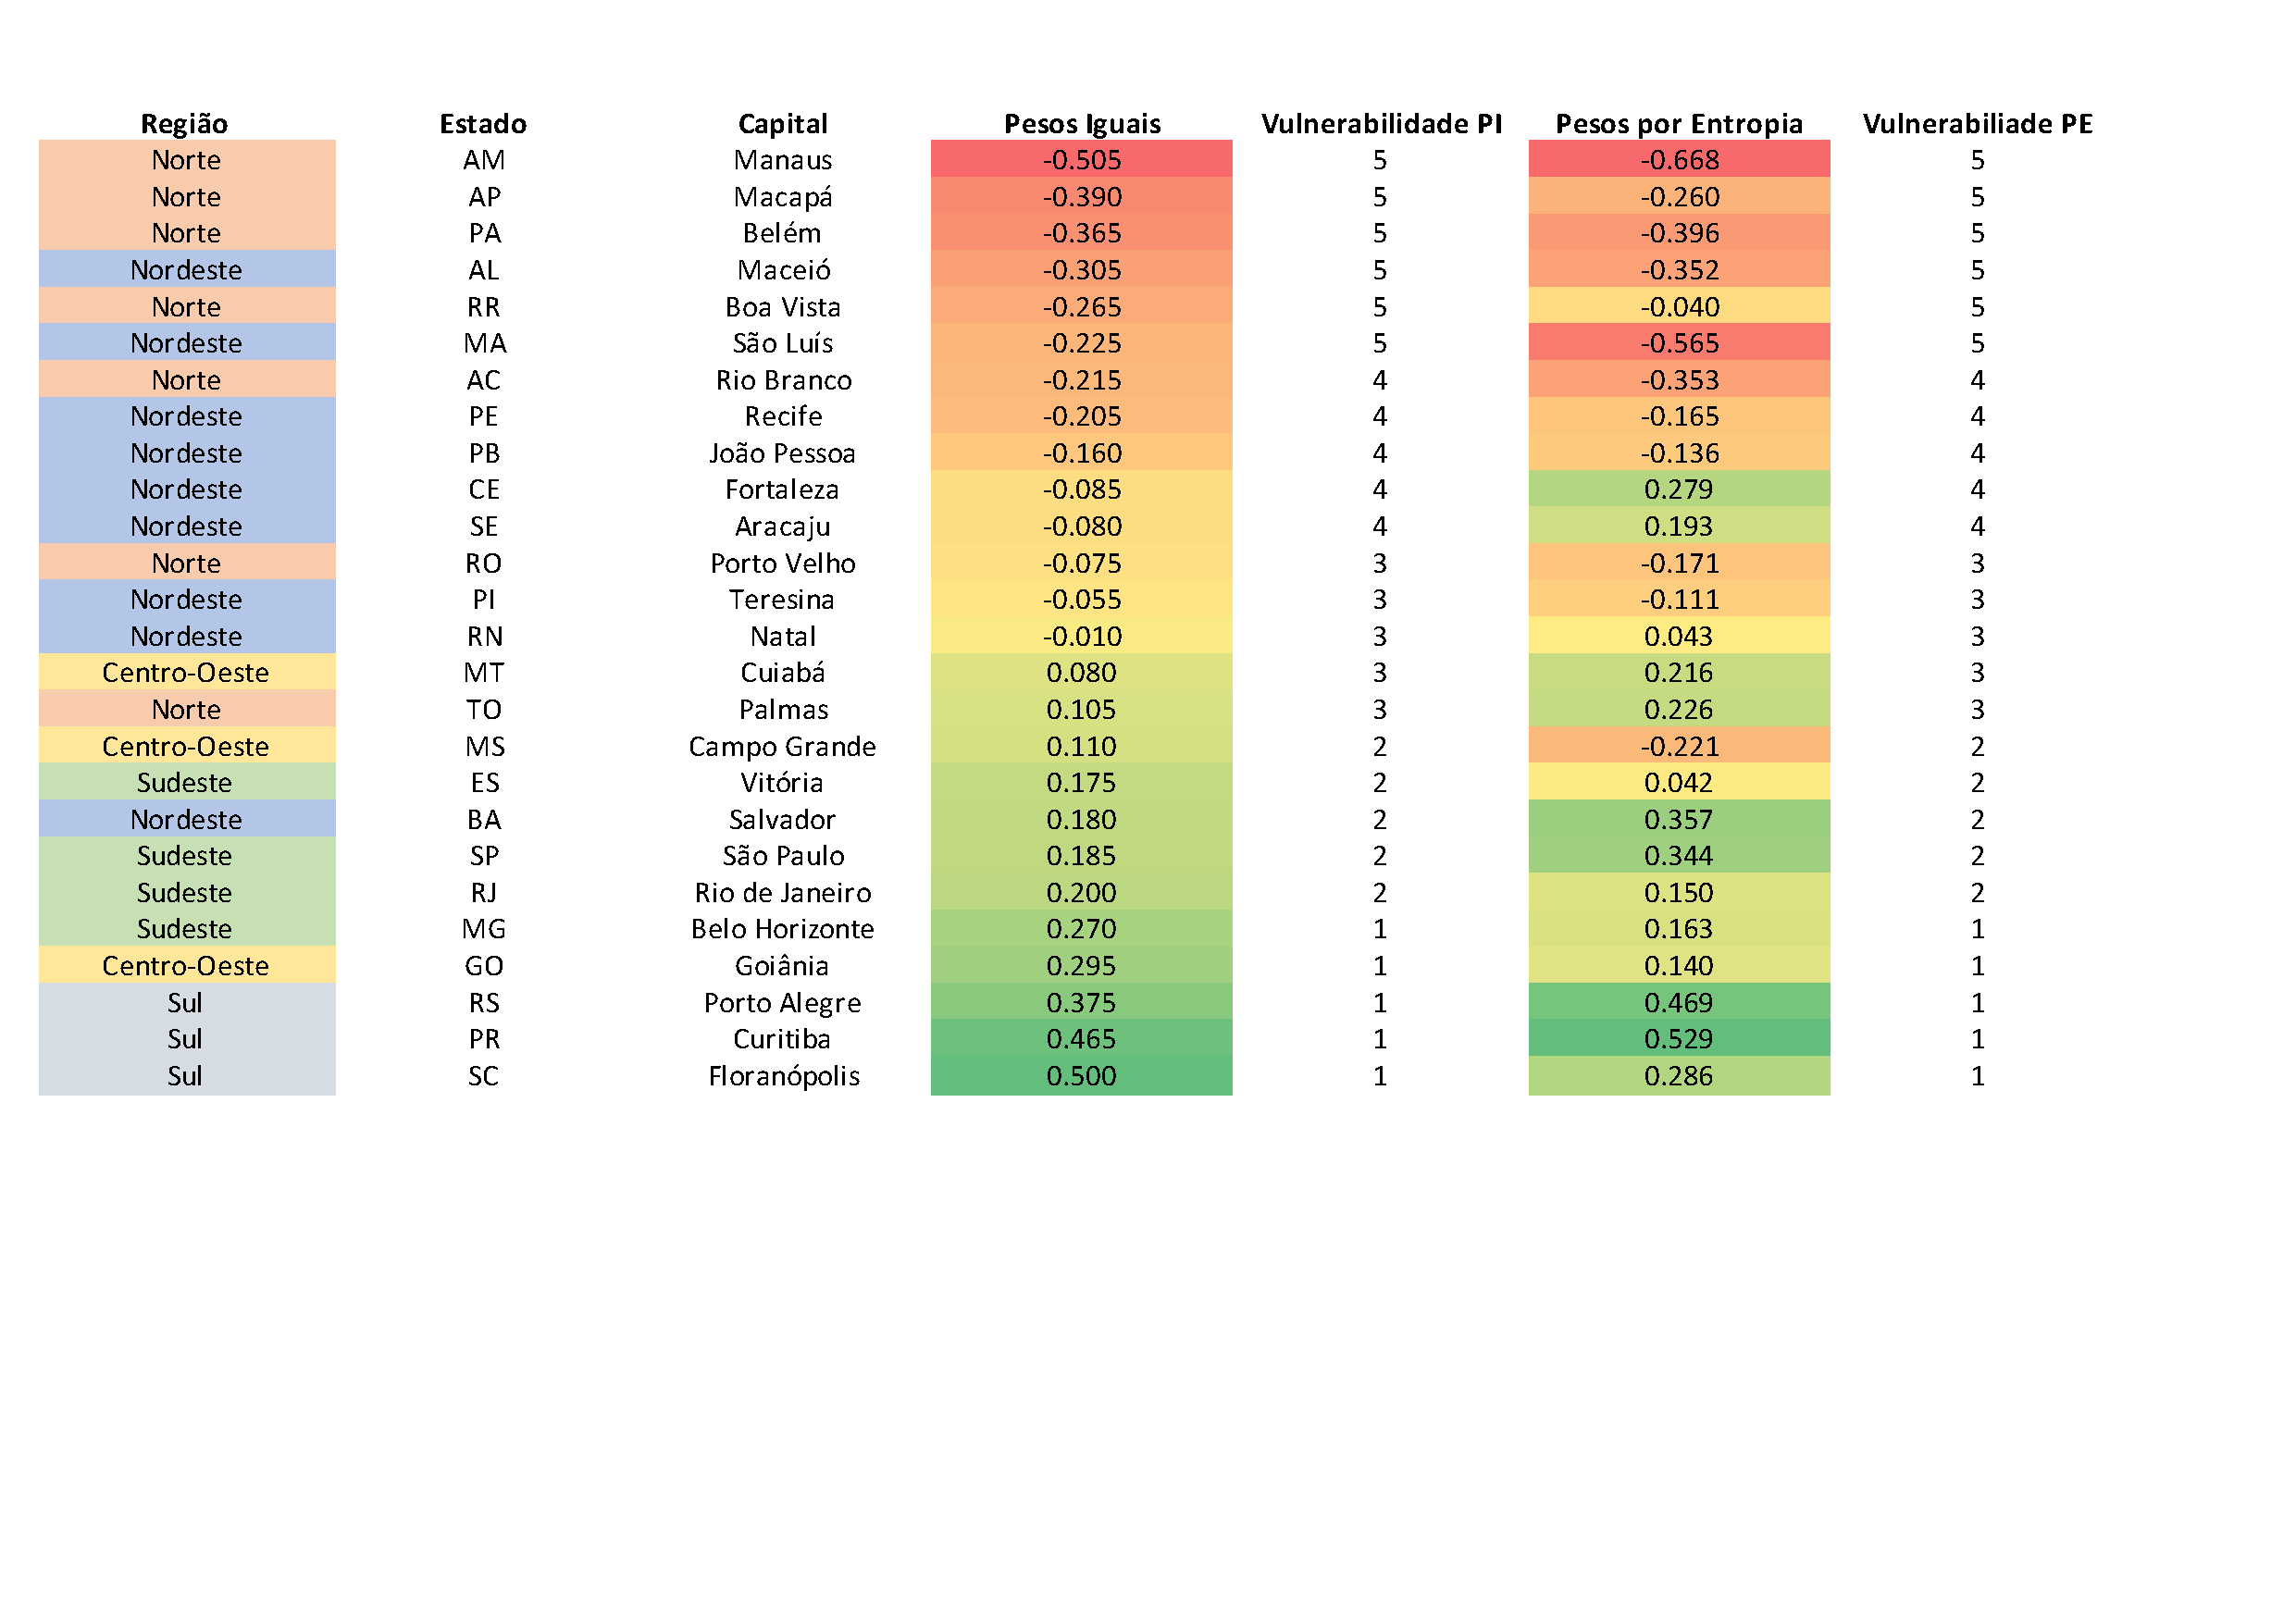
\includegraphics[width=\textwidth]{figs/resultados-iguais}
    \label{fig:resultados-iguais}
\end{figure}
	
\end{frame}

%----------------------------------------------------
\begin{frame}{Resultados}
	
\begin{columns}


\column{0.5\textwidth}
	
\begin{figure}[!h]  
	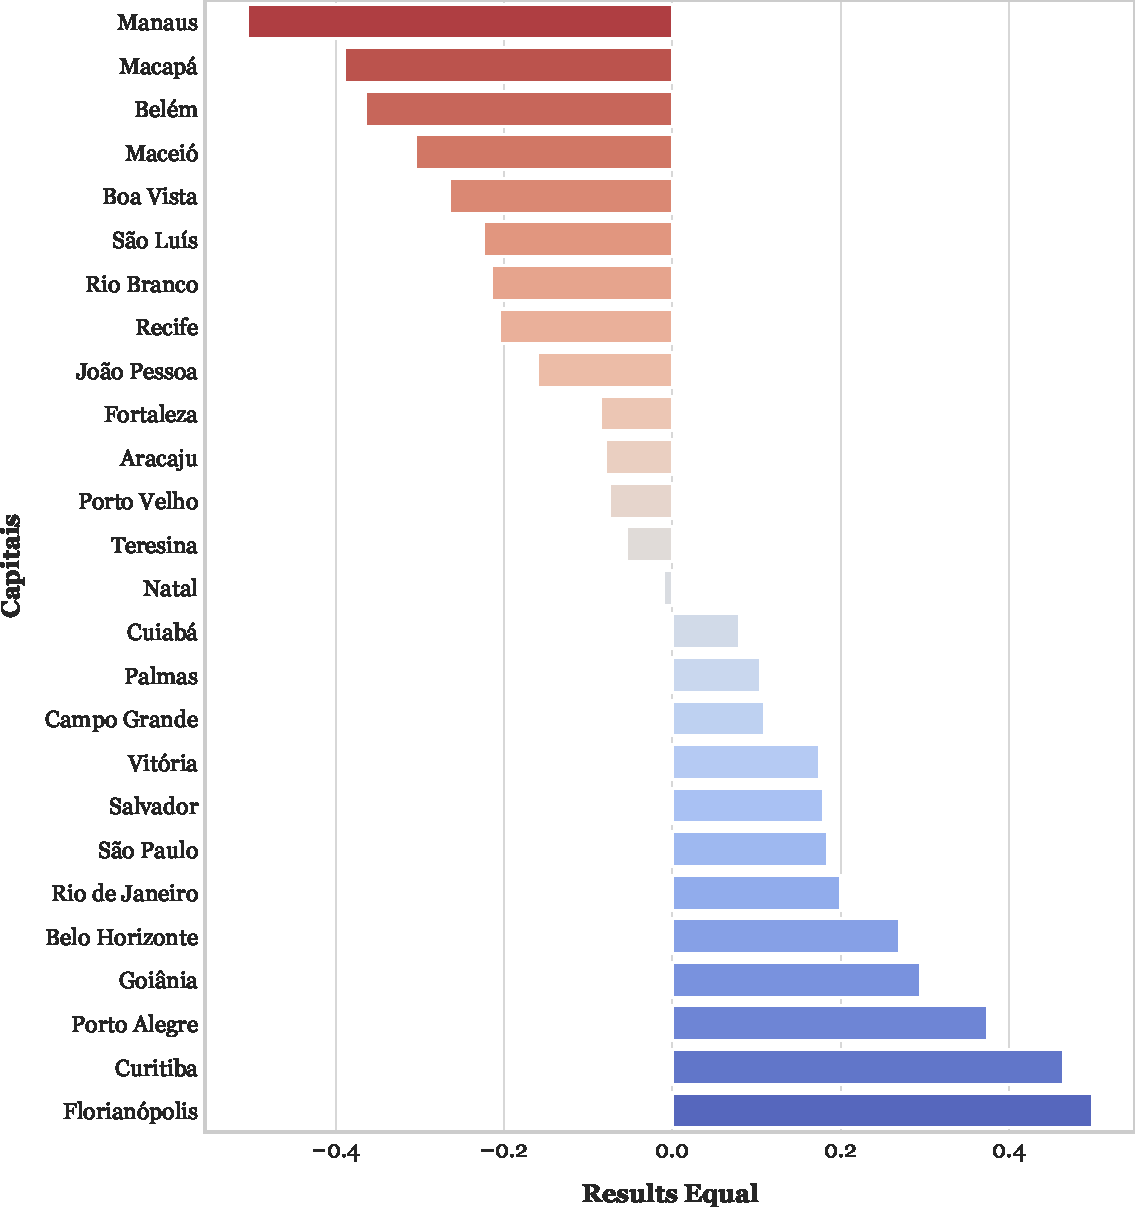
\includegraphics[width=\textwidth]{figs/barranking}
    \label{fig:bar-ranking}
\end{figure}

\column{0.45\textwidth}
	\begin{itemize}
		\item Capitais das regiões Sul e Sudeste são menos vulneráveis às consequências da pandemia;
		\item Todas as capitais com vulnerabilidade abaixo de zero são das regiões norte e nordeste;
		\item Manaus é a capital mais vulnerável do país;
		\item Florianópolis e Curitiba apresentaram menor vulnerabilidade.
	\end{itemize}
	
\end{columns}

\end{frame}

%----------------------------------------------------
\begin{frame}{Resultados por Capital - Mapa de Calor}
	
\begin{figure}[!h]  
	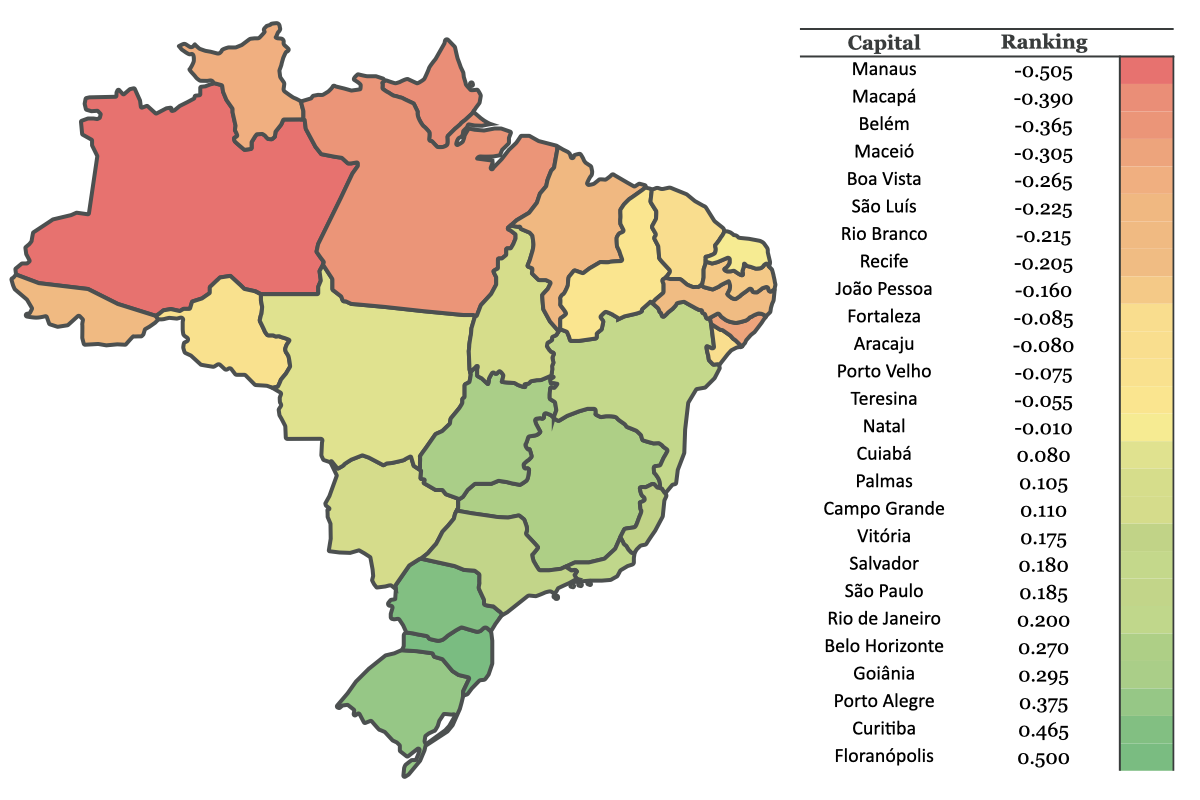
\includegraphics[width=.8\textwidth]{figs/promethee-heatmap-capitais}
    \label{fig:heatmap-capitais}
\end{figure}
	
\end{frame}

%----------------------------------------------------
\begin{frame}{Resultados por Região - Mapa de Calor}
	
\begin{figure}[!h]  
	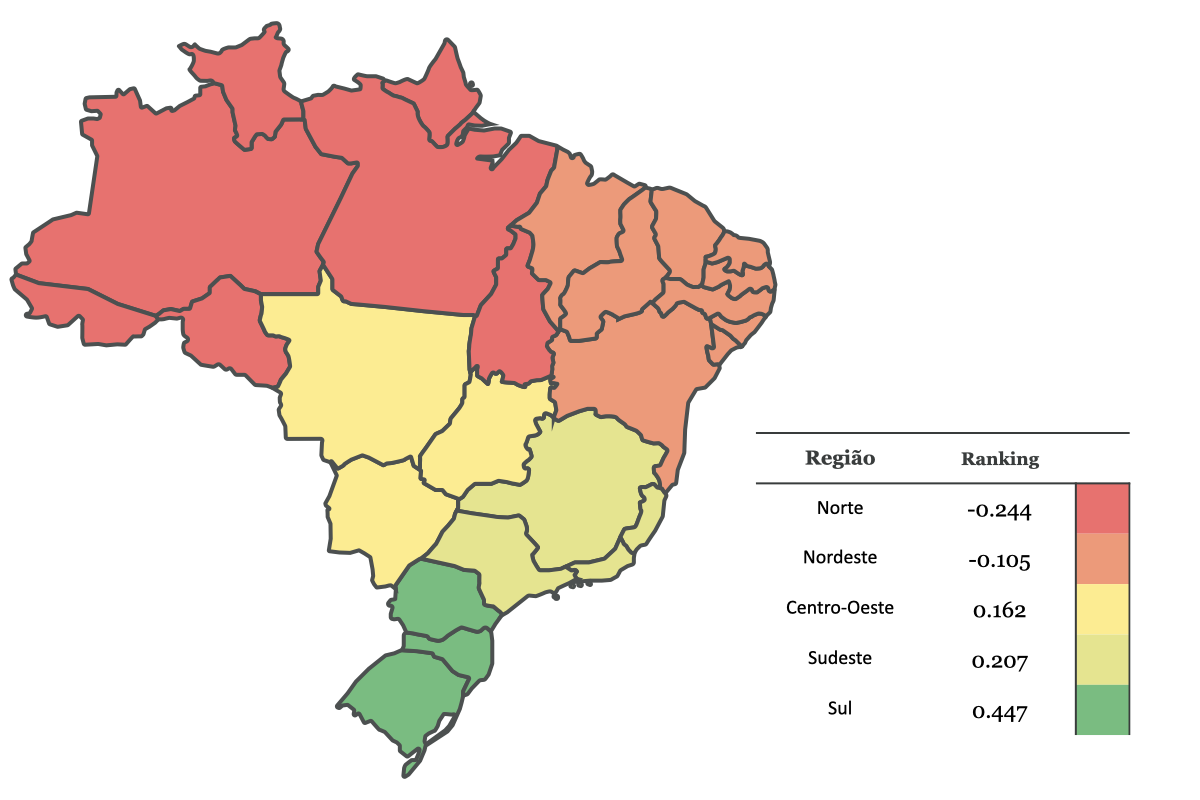
\includegraphics[width=.8\textwidth]{figs/promethee-heatmap-regiao}
    \label{fig:heatmap-regiao}
\end{figure}
	
\end{frame}

%----------------------------------------------------
\begin{frame}{Resultados}
	
\begin{itemize}
	\item As visualizações por mapa de calor reforçam a hipótese de que a pandemia atinge o país de maneira desigual;
	\item O grau de vulnerabilidade a COVID-19 é desproporcionalmente maior nas regiões Norte e Nordeste;
	\item Destaque para Manaus, a cidade que apresentou maior vulnerabilidade e que também foi retratada pela mídia como epicentro da pandemia.
	\item De forma análoga, a região Sul foi menos vulnerável e apresentou menos casos/óbitos por COVID-19 durante a pandemia.
\end{itemize}
	
\end{frame}

